\documentclass[12pt]{article}

\usepackage{graphicx}
\usepackage[a4paper,margin=1in]{geometry}
\usepackage{setspace}
\usepackage{amsmath}
\usepackage{textcomp}

\begin{document}
\noindent
\begin{minipage}{0.6\textwidth}

\includegraphics[width=0.75\textwidth]{IIITB-COMET-Logo.png}
\end{minipage}
\begin{minipage}{0.38\textwidth}
\begin{flushright}
\textbf{DARSI VAMSI}
\newline
\textbf{COMET FWC 071}
\end{flushright}
\end{minipage}
\section* {EE 2018 Q-14}
Q.In the logic circuit shown in the figure, Y is given by
\begin{center}
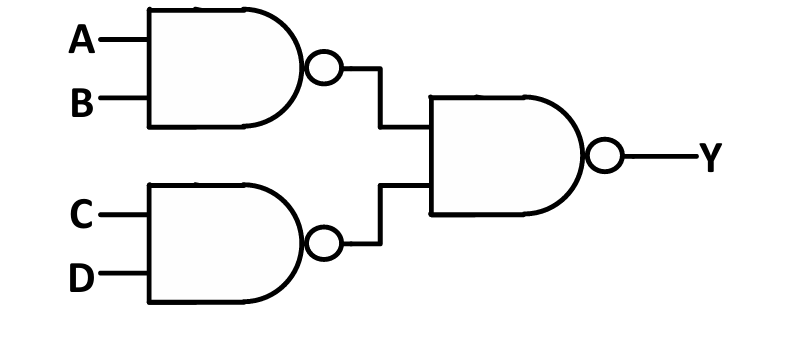
\includegraphics[width=0.75\textwidth]{figure.png}
\begin{enumerate}
\item A) $Y=ABCD$
\item B) $Y=(A+B)(C+D)$
\item C) $Y=A+B+C+D$
\item D) $Y=AB+CD$
\end{enumerate}
\end{center}
\subsection*{Step 1: First Two Gates}
The upper and lower gates are NAND gates.
\begin{equation}
X = (AB)'
\end{equation}
\begin{equation}
W = (CD)'
\end{equation}

\subsection*{Step 2: Final Gate}

The outputs of the two NAND gates are fed to another NAND gate.

\begin{equation}
Y = (XW)'
\end{equation}

Substituting $X$ and $W$,
\begin{equation}
Y = [(AB)'(CD)']'
\end{equation}

\subsection*{Step 3: Apply De Morgan's Theorem}
\begin{equation}
(A'B')' = A+B
\end{equation}

More generally,

\begin{equation}
(P'Q')' = P + Q
\end{equation}

Let

\begin{equation}
P = AB
\end{equation}

and

\begin{equation}
Q = CD
\end{equation}

Therefore,

\begin{equation}
Y = (AB) + (CD)
\end{equation}

Hence,

\begin{equation}
Y = AB + CD
\end{equation}

\subsection*{Correct Option}

\begin{equation}
\text{(D) } Y = AB + CD
\end{equation}

\end{document}
